\documentclass[tikz,border=4pt]{standalone}

% Packages
\usepackage[T1]{fontenc}
\usepackage{lmodern}
\usepackage{tikz}
\usetikzlibrary{arrows.meta, positioning, calc}

\begin{document}
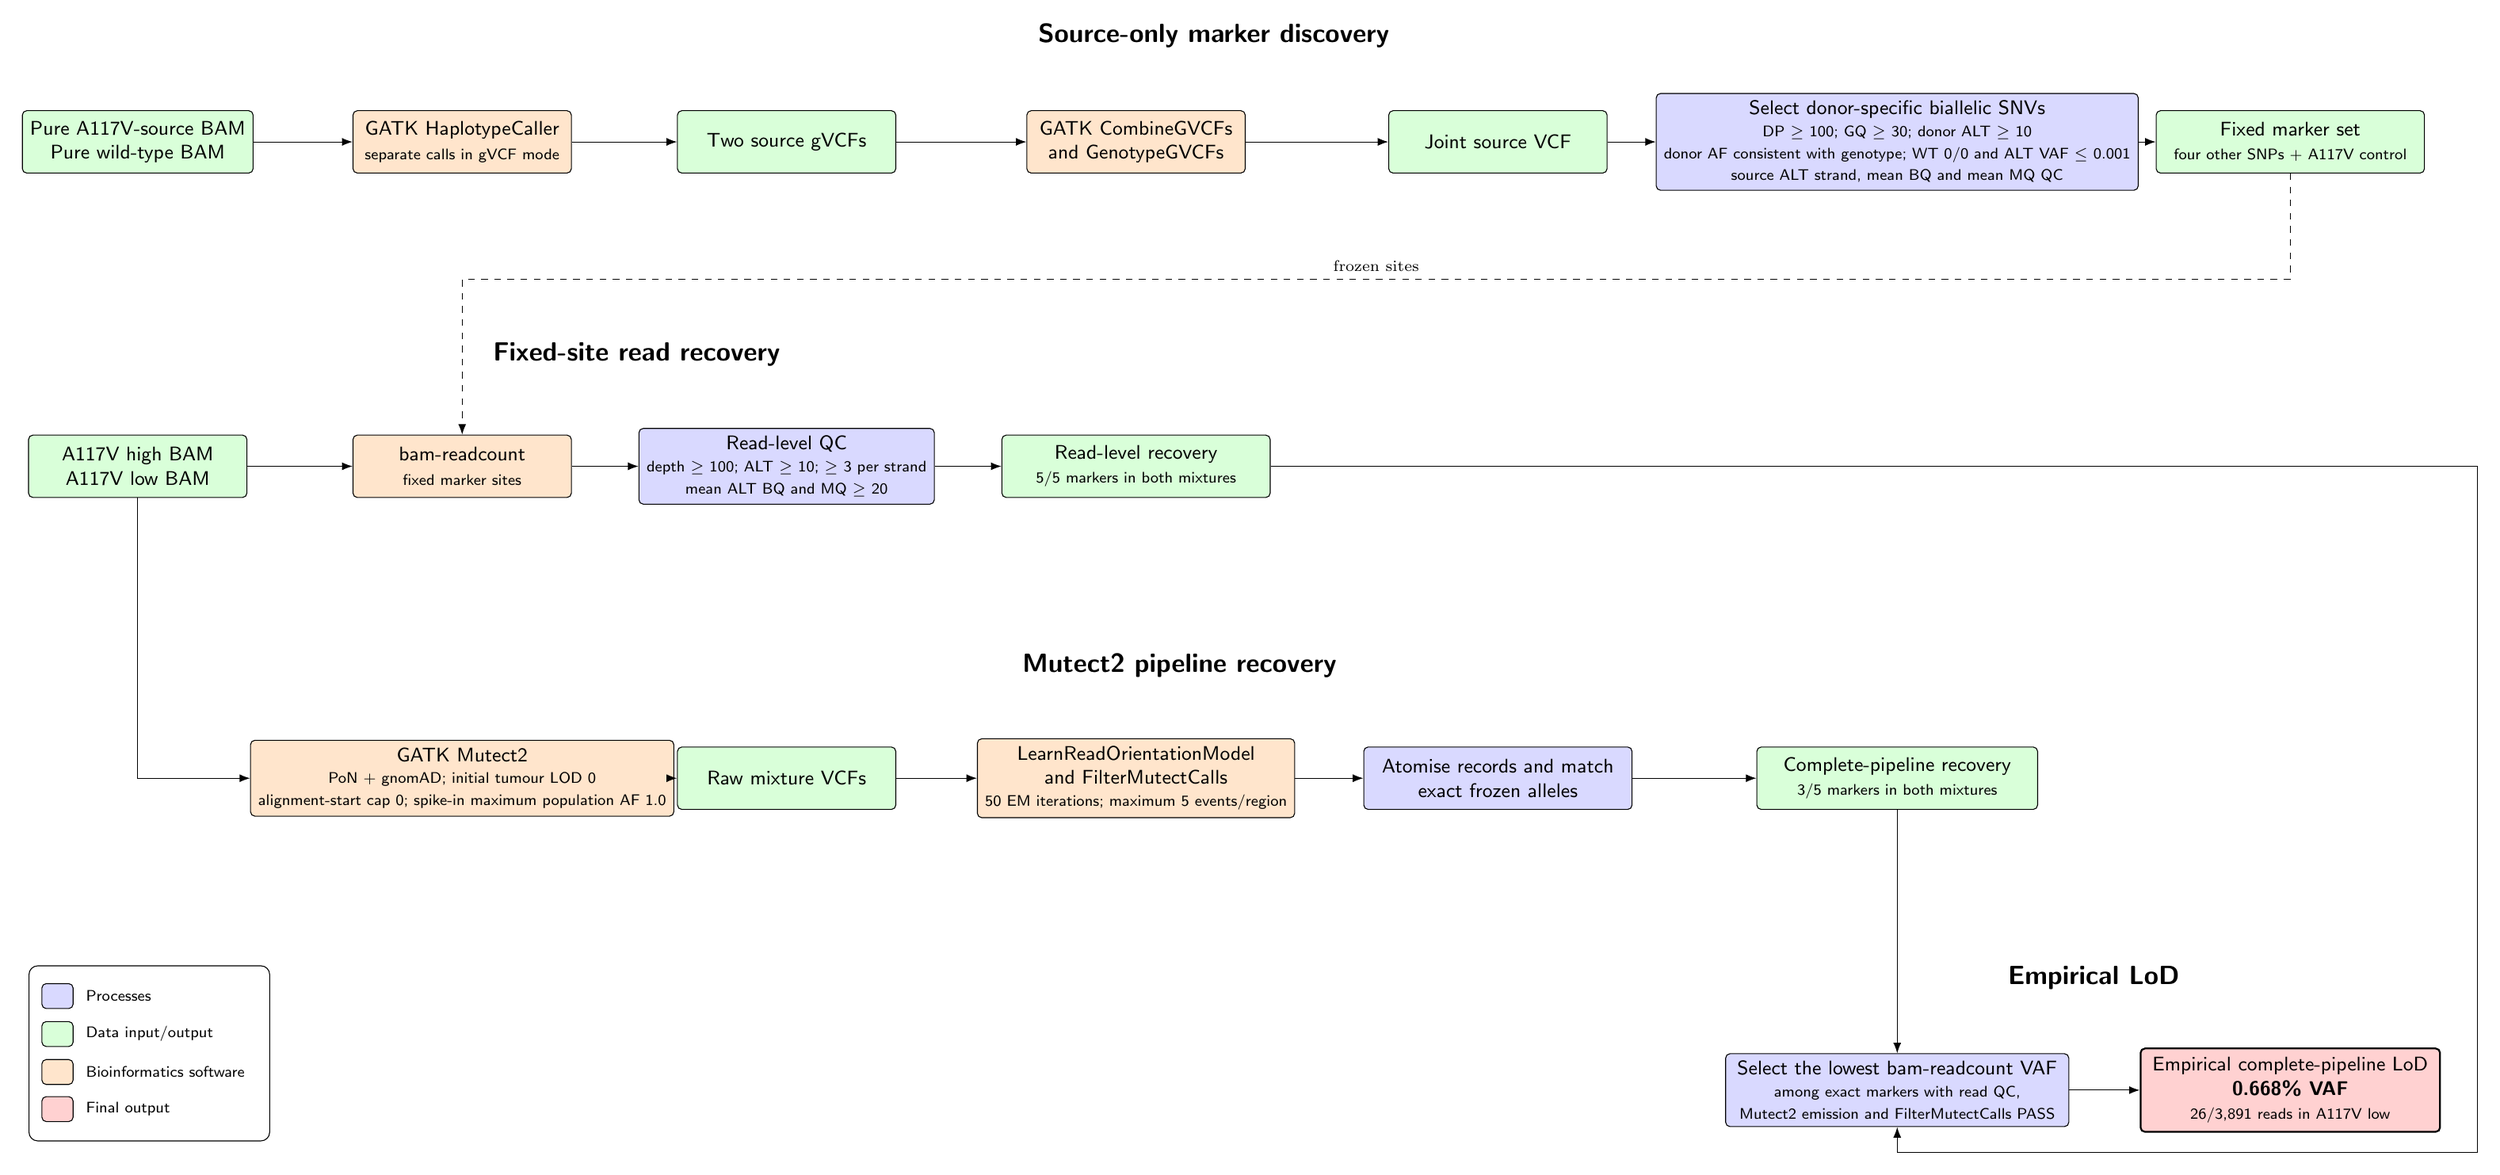
\begin{tikzpicture}[
  x=1mm,
  y=1mm,
  >=Latex,
  font=\sffamily\small,
  process/.style={draw, rounded corners=2pt, fill=blue!15, align=center,
    inner sep=3.5pt, minimum width=35mm, minimum height=10mm},
  data/.style={draw, rounded corners=2pt, fill=green!15, align=center,
    inner sep=3.5pt, minimum width=35mm, minimum height=10mm},
  software/.style={draw, rounded corners=2pt, fill=orange!20, align=center,
    inner sep=3.5pt, minimum width=35mm, minimum height=10mm},
  final/.style={draw, rounded corners=2pt, fill=red!18, align=center,
    inner sep=4pt, thick, minimum width=38mm, minimum height=12mm},
  arrow/.style={->, line width=0.4pt},
  frozenarrow/.style={->, dashed, line width=0.4pt},
  lab/.style={align=center, font=\sffamily\large, inner sep=1pt}
]

  % Define the fixed marker set from the two pure source samples only.
  \node[data] at (0,0)                             (sources) {Pure A117V-source BAM\\Pure wild-type BAM};
  \node[software] at (52,0)                        (hc)      {GATK HaplotypeCaller\\\scriptsize separate calls in gVCF mode};
  \node[data] at (104,0)                           (gvcfs)   {Two source gVCFs};
  \node[software] at (160,0)                       (joint)   {GATK CombineGVCFs\\and GenotypeGVCFs};
  \node[data] at (218,0)                           (jointvcf){Joint source VCF};
  \node[process, minimum width=56mm] at (282,0)    (select) {
    Select donor-specific biallelic SNVs\\[-1pt]
    \scriptsize DP $\geq$ 100; GQ $\geq$ 30; donor ALT $\geq$ 10\\[-1pt]
    \scriptsize donor AF consistent with genotype; WT 0/0 and ALT VAF $\leq$ 0.001\\[-1pt]
    \scriptsize source ALT strand, mean BQ and mean MQ QC};
  \node[data, minimum width=43mm] at (345,0)        (markers) {Fixed marker set\\\scriptsize four other SNPs + A117V control};

  \draw[arrow] (sources)  -- (hc);
  \draw[arrow] (hc)       -- (gvcfs);
  \draw[arrow] (gvcfs)    -- (joint);
  \draw[arrow] (joint)    -- (jointvcf);
  \draw[arrow] (jointvcf) -- (select);
  \draw[arrow] (select)   -- (markers);

  % Interrogate the frozen sites directly in both mixtures.
  \node[data] at (0,-52)                           (mixtures) {A117V high BAM\\A117V low BAM};
  \node[software] at (52,-52)                      (readcount){bam-readcount\\\scriptsize fixed marker sites};
  \node[process, minimum width=47mm] at (104,-52)  (readqc) {
    Read-level QC\\[-1pt]
    \scriptsize depth $\geq$ 100; ALT $\geq$ 10; $\geq$ 3 per strand\\[-1pt]
    \scriptsize mean ALT BQ and MQ $\geq$ 20};
  \node[data, minimum width=43mm] at (160,-52)     (readpass) {Read-level recovery\\\scriptsize 5/5 markers in both mixtures};

  \draw[arrow] (mixtures)  -- (readcount);
  \draw[arrow] (readcount) -- (readqc);
  \draw[arrow] (readqc)    -- (readpass);
  \coordinate (markerbranch) at (345,-22);
  \draw[dashed, line width=0.4pt] (markers.south) -- (markerbranch);
  \draw[frozenarrow] (markerbranch) -- node[above, font=\scriptsize] {frozen sites}
    (52,-22) -- (readcount.north);

  % Assess the same markers through Mutect2 and FilterMutectCalls.
  \node[software, minimum width=50mm] at (52,-102) (mutect) {
    GATK Mutect2\\[-1pt]
    \scriptsize PoN + gnomAD; initial tumour LOD 0\\[-1pt]
    \scriptsize alignment-start cap 0; spike-in maximum population AF 1.0};
  \node[data] at (104,-102)                        (rawvcf)   {Raw mixture VCFs};
  \node[software, minimum width=48mm] at (160,-102)(filter) {
    LearnReadOrientationModel\\and FilterMutectCalls\\[-1pt]
    \scriptsize 50 EM iterations; maximum 5 events/region};
  \node[process, minimum width=43mm] at (218,-102) (match)    {Atomise records and match\\exact frozen alleles};
  \node[data, minimum width=45mm] at (282,-102)    (complete) {Complete-pipeline recovery\\\scriptsize 3/5 markers in both mixtures};

  \draw[arrow] (mixtures.south) -- (0,-102) -- (mutect.west);
  \draw[arrow] (mutect)   -- (rawvcf);
  \draw[arrow] (rawvcf)   -- (filter);
  \draw[arrow] (filter)   -- (match);
  \draw[arrow] (match)    -- (complete);

  % Derive the complete-pipeline LoD from the count-based VAF.
  \node[process, minimum width=55mm] at (282,-152) (lodselect) {
    Select the lowest bam-readcount VAF\\[-1pt]
    \scriptsize among exact markers with read QC,\\[-1pt]
    \scriptsize Mutect2 emission and FilterMutectCalls PASS};
  \node[final, minimum width=48mm] at (345,-152)   (lod)      {Empirical complete-pipeline LoD\\\textbf{0.668\% VAF}\\\scriptsize 26/3,891 reads in A117V low};

  \draw[arrow] (readpass.east) -- (375,-52) -- (375,-162) --
    (282,-162) -- (lodselect.south);
  \draw[arrow] (complete.south) -- (lodselect.north);
  \draw[arrow] (lodselect) -- (lod);

  % Section titles clarify that mixture evidence cannot affect marker selection.
  \node[lab] at (172.5,17)  {\textbf{Source-only marker discovery}};
  \node[lab] at (80,-34)    {\textbf{Fixed-site read recovery}};
  \node[lab] at (167,-84)   {\textbf{Mutect2 pipeline recovery}};
  \node[lab] at (313.5,-134){\textbf{Empirical LoD}};

  % Compact colour key matching the main analytical workflow figure.
  \matrix[anchor=north west, draw, rounded corners, inner sep=2mm, fill=white]
    at (-17.5,-132)
  {
    \node[anchor=center, draw, rounded corners=2pt, fill=blue!15, minimum width=5mm, minimum height=4mm] {}; & \node[anchor=west, align=left]{\scriptsize Processes}; \\
    \node[anchor=center, draw, rounded corners=2pt, fill=green!15, minimum width=5mm, minimum height=4mm] {}; & \node[anchor=west, align=left]{\scriptsize Data input/output}; \\
    \node[anchor=center, draw, rounded corners=2pt, fill=orange!20, minimum width=5mm, minimum height=4mm] {}; & \node[anchor=west, align=left]{\scriptsize Bioinformatics software}; \\
    \node[anchor=center, draw, rounded corners=2pt, fill=red!18, minimum width=5mm, minimum height=4mm] {}; & \node[anchor=west, align=left]{\scriptsize Final output}; \\
  };

\end{tikzpicture}
\end{document}
